\documentclass{article}
\usepackage[dblblindworkshop,final]{neurips_2026}
\usepackage[utf8]{inputenc}
\usepackage[T1]{fontenc}
\usepackage{hyperref}
\hypersetup{hidelinks}
\usepackage{url}
\usepackage{booktabs}
\usepackage{array}
\usepackage{amsmath}
\usepackage{amssymb}
\usepackage{graphicx}
\usepackage{microtype}
\usepackage{caption}
\usepackage{float}
\usepackage{xcolor}
\newcommand{\TODO}[1]{\textcolor{red}{\textbf{[TODO: #1]}}}
\captionsetup{font=small,labelfont=bf}
\newcommand{\ci}[2]{{\footnotesize[#1,\,#2]}}
\newcommand{\best}[1]{\textbf{#1}}
\graphicspath{{figures/}}

\title{Can an Injected-Failure Benchmark Pick Your Monitor?\\
A Four-Part Validity Audit for Enterprise Agent Deployment}
\workshoptitle{AABA4ET: Agentic AI Benchmarks and Applications for Enterprise Tasks}
\author{%
  Dev Utkarsh Pal\\ \TODO{affiliation}\\ \texttt{\TODO{email}}
  \And
  Arpan Verma\\ \TODO{affiliation}\\ \texttt{\TODO{email}}
  \And
  Chandan Sah\\ \TODO{affiliation}\\ \texttt{\TODO{email}}
  \And
  Aditya Upadhyay\\ \TODO{affiliation}\\ \texttt{\TODO{email}}
  \And
  Harshit Gupta\\ \TODO{affiliation}\\ \texttt{\TODO{email}}
}
\begin{document}
\maketitle
\begin{abstract}
An enterprise that runs agents in production needs to detect when one fails, and it usually
picks the monitor that scores best on a benchmark of labelled failures. Those labels are cheap
to obtain by injection: change a step of a successful trajectory and the benchmark knows which
step it changed. A correct label, however, does not show that the injected failure stands in
for the failures the monitor will meet in service. We treat the injector as part of the
evaluation and ask four questions. Can a detector read data written only by the injector? When
two methods create the same error, can it tell which method was used? On the same task, can it
tell injected and natural failures apart? Would injected and natural data lead us to pick the
same monitor? On 24,000 agent traces the four tests give different answers. Removing
injector-only data erases some apparent detection ability. One injection method stays
identifiable after we control measured error severity. Matching on the query removes an
apparent realism trend, and the monitor chosen from injected data changes with the detector
set. The gap matters at deployment: a monitor selected on injected traces can lose measurable
accuracy under the shift to natural failures. The audit gives enterprise benchmark builders a
practical way to state which claims their injected failures support before a monitor goes into
production. Code, results and traces are available at
\url{https://github.com/deecod-dev/mirage}.
\end{abstract}

\section{Why a clear label is not enough to pick a monitor}
An agent running an enterprise workflow fails in ways nobody watches in real time, so teams attach an automatic monitor and choose it by how well it scores on a benchmark of labelled failures. Building that benchmark is the hard part: a failed trajectory records what happened but does not identify the step that caused the outcome. AEGIS, Who\&When Pro, and AgenTracer therefore change successful
trajectories and use the changed step as the label \citep{aegis,whenpro,agentracer}. This gives
a clear label without finding the cause afterward.

The injected failure may still differ from a natural one. For example, a benchmark may know
which supporting passage it removed, while the replacement rule leaves an obvious marker. A
detector can then score well for the wrong reason. Prior work studies whether benchmarks
measure their intended concept \citep{bean} and shows gaps between synthetic and natural data
\citep{chwang,rethinking,ragsynth}. We turn these concerns into four tests for injected agent
benchmarks:
\begin{description}\itemsep0pt
\item[V1 Independence:] Can the detector read data written only by the injector?
\item[V2 Mechanism signal:] When two methods create the same error, can the detector tell
which method was used?
\item[V3 Natural match:] On the same task, can it tell injected and natural failures apart?
\item[V4 Detector choice:] Would injected and natural data lead us to choose the same detector,
and how much natural-data performance is lost if they do not?
\end{description}

\begin{figure}[t]
\centering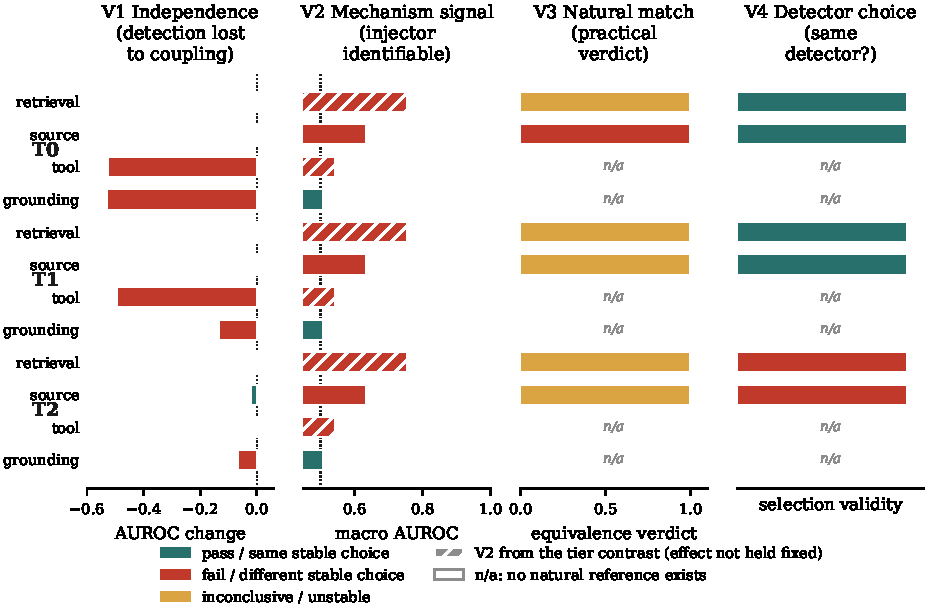
\includegraphics[width=\textwidth]{fig1_validity_matrix.pdf}
\caption{The four tests give different answers on the same benchmark conditions. Undefined
and inconclusive cells are not counted as passes.}
\label{fig:matrix}
\end{figure}

\section{Experimental setup}
The agent pipeline uses BGE retrieval and reranking, Qwen2.5-7B-Instruct for generation and
judging, and real tool execution. The main dataset contains $24{,}000$ HotpotQA and GSM8K
traces. We inject four kinds of failures involving the query, supporting sources, tool use,
and final answer. Each has naive (T0), literature-inspired (T1), and artifact-hardened (T2)
versions. Three of fourteen detector features read injector-written data directly; the main
feature set removes them. Training and test folds never share a query. We use 1,000
query-level bootstrap samples for uncertainty.

HotpotQA labels which passages support an answer. We call a trace a naturally occurring
retrieval degradation when the selected context omits a required passage. A separate 2Wiki
run adds $7{,}000$ traces, including 521 natural degradations and 6,000 injected traces on the
same queries.

\section{Results}
\paragraph{V1: injector-only data can inflate scores.} Tool-fault detection at T1 falls from
$.990$ to $.495$ after removing the three direct links; tool T0 falls from $1.000$ to $.473$,
and grounding T0 from $1.000$ to $.469$. Retrieval T1 ($.864$) and source T1 ($.963$) change
little. The losses are therefore tied to the direct links rather than a general loss of signal.

\begin{figure}[t]
\centering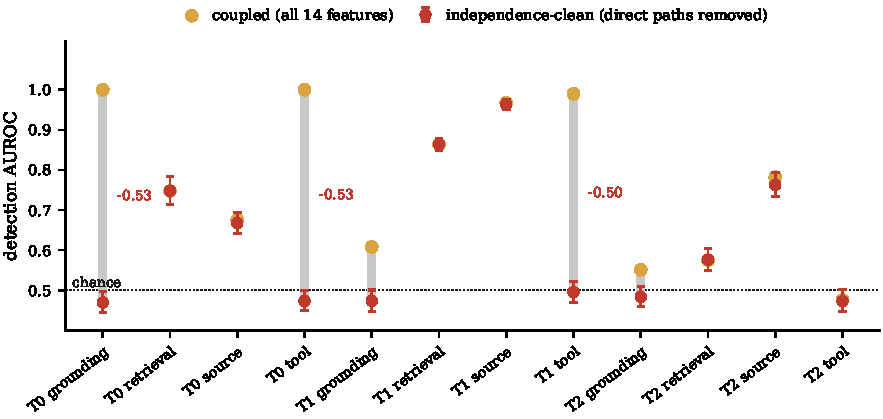
\includegraphics[width=\textwidth]{fig2_coupling_collapse.pdf}
\caption{Detection AUROC before and after removing features that directly read injector data.
Large losses occur only in conditions with a direct link.}
\label{fig:v1-short}
\end{figure}

\paragraph{V2: the injection method can leave a signal.}\label{sec:artifact} Two source
injectors replace one supporting passage in the same slot with a rejected passage from the
same query. A classifier identifies which method was used with AUROC $.633$
\ci{.601}{.664}. Measured error severity explains part of this result. After reweighting eight
severity measures, the classifier still reaches $.607$ \ci{.576}{.639}. A similar grounding
comparison is at chance ($.504$). The signal therefore appears for one tested fault type but
not the other.

\begin{figure}[t]
\centering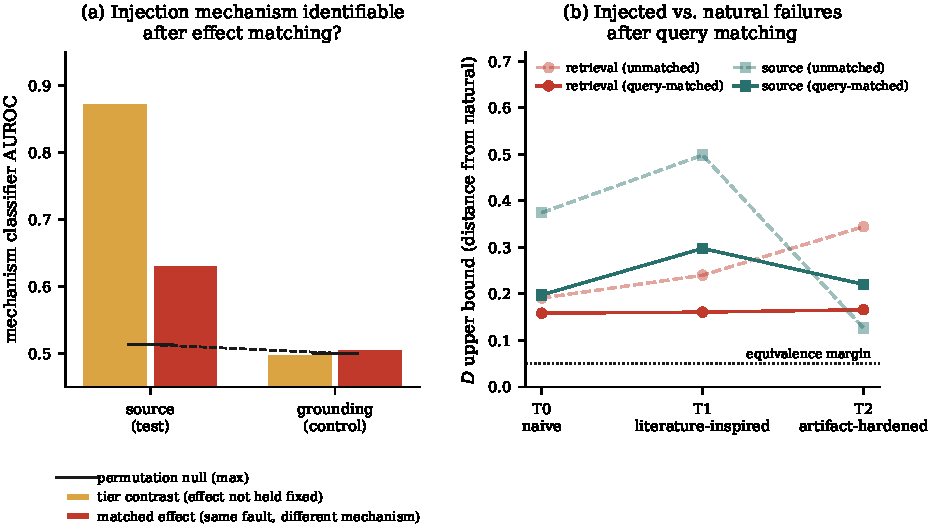
\includegraphics[width=\textwidth]{fig3_artifact_ecological.pdf}
\caption{(a) Can a classifier identify the injection method after the intended error is
matched? (b) Can it tell injected and natural failures apart on the same queries?}
\label{fig:v23}
\end{figure}

\paragraph{V3: the query must be matched.}\label{sec:ecological} Without matching, source
faults appear closer to natural failures as the injector is hardened, while retrieval faults
move the other way. Natural failures, however, occur on queries the retriever finds hard. The
pattern disappears when injected and natural traces use the same queries. No Hotpot condition
establishes a practical match at $\delta=.05$; most results are inconclusive rather than proven
different. On 2Wiki, all six conditions are distinguishable, but hardening still has no steady
direction.

\paragraph{V4: the detector set changes the answer.} With all seven detectors, Hotpot T0/T1
choose the natural-data winner. T2 chooses a different detector but loses only $.004$ AUROC on
natural data. After removing detectors that fail V1, T0/T1 lose $.058$, while T2 chooses the
same detector in $.990$ of bootstrap samples. On 2Wiki, the V1-clean T0/T2 choices lose $.088$
\ci{.059}{.115}. Detector choice therefore depends on the benchmark, natural data, metric,
and detectors being compared.

\section{Checking the natural comparison}
We add the missing gold passage back to wrong-answer traces and rerun the agent. On HotpotQA,
$.311$ of answers become correct, compared with $.100$ when we add a different non-gold
passage of similar length. On 2Wiki, the rates are $.332$ and $.107$. Missing evidence
therefore contributes to some wrong answers, but it is not a complete cause label for every
case. On 600 released AEGIS traces, removing available injector fields changes AUROC by $.032$
\ci{.001}{.066} and $.022$ \ci{-.011}{.058} for two modes. Both intervals cross the $.05$
margin, so these external V1 results are inconclusive.

\section{A protocol for enterprise benchmark builders}
Before using injected failures to compare detectors: (1) remove direct paths from injector
data to the detector; (2) build two methods that create the same error and test whether the
method can be identified; (3) compare injected and natural failures on the same tasks; (4)
check whether both sources choose the same detector and report the natural-data loss when they
do not; and (5) report undefined or inconclusive tests instead of treating them as passes.
For an enterprise deployment, step (4) carries the cost: a monitor chosen on injected traces
can lose measurable accuracy under the shift to the natural failures it meets in service.

\begin{table}[t]
\centering\scriptsize
\caption{Each benchmark claim needs different evidence. A failed or inconclusive test limits
only the claim in its row.}
\begin{tabular}{@{}lp{4.1cm}p{4.1cm}@{}}
\toprule
Claim & Required evidence & Evidence here \\
\midrule
Score does not use injector-only data & V1 after direct links are removed & passes for several
retrieval/source cells; fails for three coupled cells \\
Injection method does not matter & V2 after matching the error and severity & source signal
remains; grounding is at chance \\
Injected failures match natural ones & V3 on the same queries & no practical match at
$\delta=.05$ on either dataset \\
Injected data choose the natural-data detector & V4 choice stability and natural-data loss &
answer changes with dataset and detector set \\
\bottomrule
\end{tabular}
\label{tab:claim-evidence-short}
\end{table}

\paragraph{Limits and conclusion.}
The study uses one agent pipeline and one generator. Natural comparisons exist only for
retrieval-side faults, and V2 matches the intended error for only two of four fault types.
Failure to identify a difference under the tested features does not prove that the full trace
distributions are equal. The appendix gives the complete settings, features, injector
operations, uncertainty results, and second-dataset tables. \textbf{Clear injected labels are useful, but a benchmark that has not been
audited cannot tell an enterprise which monitor to trust in production.}

\acksection
\TODO{acknowledgements and funding disclosure, or ``The authors declare no funding or competing interests.''}

\clearpage
\bibliographystyle{plainnat}
\begin{thebibliography}{99}
\small

\bibitem[Bean et al.(2025)]{bean}
A.~M. Bean et al.
\newblock Measuring what matters: Construct validity in large language model benchmarks.
\newblock In \emph{NeurIPS Datasets and Benchmarks}, 2025.

\bibitem[Kong et al.(2026)]{aegis}
F.~Kong et al.
\newblock Aegis: Automated error generation and attribution for multi-agent systems.
\newblock In \emph{ICLR}, 2026.

\bibitem[Jia et al.(2026)]{masfire}
J.~Jia, Z.~Deng, Z.~Chen, Y.~Wang, and Z.~Zheng.
\newblock {MAS-FIRE}: Fault injection and reliability evaluation for {LLM}-based multi-agent systems.
\newblock \emph{arXiv:2602.19843}, 2026.

\bibitem[Tan et al.(2026)]{agentchaos}
G.~Tan et al.
\newblock {AgentChaos}: Chaos engineering for agent systems via programmatic fault injection.
\newblock \emph{arXiv:2608.06790}, 2026.

\bibitem[Yu et al.(2026)]{fisurvey}
G.~Yu, G.~Tan, H.~Huang, Z.~Zhang, P.~Chen, R.~Natella, and Z.~Zheng.
\newblock A survey on failure analysis and fault injection in {AI} systems.
\newblock \emph{ACM Transactions on Software Engineering and Methodology}, 35(1):28:1--28:42,
2026.

\bibitem[Chen et al.(2026)]{rethinking}
W.~Chen, V.~Padmanabhan, T.~Giyahchi, E.~Wong, and L.~Akoglu.
\newblock Rethinking evaluation for {LLM} hallucination detection: A desiderata, a new {RAG}-based benchmark, new insights.
\newblock In \emph{ACL}, 2026.

\bibitem[CH-Wang et al.(2024)]{chwang}
S.~CH-Wang, B.~Van~Durme, J.~Eisner, and C.~Kedzie.
\newblock Do androids know they're only dreaming of electric sheep?
\newblock In \emph{Findings of ACL}, 2024.

\bibitem[Deshpande et al.(2025)]{trail}
D.~Deshpande et al.
\newblock {TRAIL}: Trace reasoning and agentic issue localization.
\newblock \emph{arXiv:2505.08638}, 2025.

\bibitem[Es et al.(2024)]{ragas}
S.~Es, J.~James, L.~Espinosa-Anke, and S.~Schockaert.
\newblock {RAGAS}: Automated evaluation of retrieval augmented generation.
\newblock In \emph{EACL}, 2024.

\bibitem[Geirhos et al.(2020)]{geirhos}
R.~Geirhos et al.
\newblock Shortcut learning in deep neural networks.
\newblock \emph{Nature Machine Intelligence}, 2(11):665--673, 2020.

\bibitem[Gururangan et al.(2018)]{gururangan}
S.~Gururangan, S.~Swayamdipta, O.~Levy, R.~Schwartz, S.~R. Bowman, and N.~A. Smith.
\newblock Annotation artifacts in natural language inference data.
\newblock In \emph{NAACL-HLT}, 2018.

\bibitem[Liu et al.(2026)]{whenpro}
J.~Liu et al.
\newblock Who\&{W}hen {P}ro: Can {LLM}s really attribute failures in {AI} agents?
\newblock \emph{arXiv:2607.09996}, 2026.

\bibitem[Manakul et al.(2023)]{selfcheckgpt}
P.~Manakul, A.~Liusie, and M.~J.~F. Gales.
\newblock {SelfCheckGPT}: Zero-resource black-box hallucination detection for generative large language models.
\newblock In \emph{EMNLP}, 2023.

\bibitem[McCoy et al.(2019)]{hans}
R.~T. McCoy, E.~Pavlick, and T.~Linzen.
\newblock Right for the wrong reasons: Diagnosing syntactic heuristics in natural language inference.
\newblock In \emph{ACL}, 2019.

\bibitem[Niu et al.(2024)]{ragtruth}
C.~Niu et al.
\newblock {RAGTruth}: A hallucination corpus for developing trustworthy retrieval-augmented language models.
\newblock In \emph{ACL}, 2024.

\bibitem[Saad-Falcon et al.(2024)]{ares}
J.~Saad-Falcon, O.~Khattab, C.~Potts, and M.~Zaharia.
\newblock {ARES}: An automated evaluation framework for retrieval-augmented generation systems.
\newblock In \emph{NAACL}, 2024.

\bibitem[van Elburg et al.(2025)]{ragsynth}
J.~van Elburg, P.~van der Putten, and M.~Marx.
\newblock Can we evaluate {RAG}s with synthetic data?
\newblock In \emph{SynDAiTE Workshop at ECML-PKDD}, 2025.

\bibitem[Zhang et al.(2025)]{agentracer}
G.~Zhang et al.
\newblock {AgenTracer}: Who is inducing failure in the {LLM} agentic systems?
\newblock \emph{arXiv:2509.20846}, 2025.

\end{thebibliography}

\appendix

\section{Operating-point and second-dataset details}
\label{app:k3}

\paragraph{HotpotQA $k{=}3$.} Because $k{=}2$ was chosen after inspecting the natural-failure
rate, we repeat the natural and decision analyses at $k{=}3$. Natural failures fall to
$17.25\%$ ($138/800$), while wrongness lift remains positive at $+0.292$
\ci{+0.205}{+0.374}. Under Set~A, T0/T1 agree and T2 misselects (regret $0.015$, bootstrap
agreement $.038$); under Set~B, T0/T1 misselect while T2 agrees only unstably
($P_{\rm agree}=.573$). The qualitative candidate-pool interaction survives the operating
point, but its individual point winners need not be stable.

\paragraph{2Wiki protocol.} A 200-query validation pilot, excluded from all later analysis,
observed $114$ natural degradations and projected $570$ at the fixed cap of $1{,}000$. The
confirmatory partition contains exactly $1{,}000$ clean and $6{,}000$ synthetic traces:
T0--T2 crossed with retrieval and source degradation. Query-disjoint five-fold predictions,
within-query permutation nulls and $1{,}000$ query-cluster bootstraps are unchanged from the
primary protocol. Both partitions use the \texttt{framolfese/2WikiMultihopQA} validation
split with seed \texttt{20260823}. Among the $521$ confirmatory natural degradations, $302$
omit one annotated supporting title and $219$ omit multiple ($213$ omit two and $6$ omit
three); their wrong-answer rates are $.517$, $.141$, and $.167$, respectively. We therefore
retain the missing-evidence count as a severity descriptor rather than interpreting the
pooled natural class as severity-homogeneous.

\begin{table}[h]
\centering\scriptsize
\caption{Full 2Wiki decision-validity replication. Regret is measured on natural failures;
intervals and $P_{\rm agree}$ use query-cluster bootstrap resamples.}
\label{tab:2wiki-v4}
\begin{tabular}{@{}lllccl@{}}
\toprule
Set & Tier & Synthetic choice & Natural choice & $P_{\rm agree}$ & Regret [95\% CI] \\
\midrule
All & T0 & all features & all features & .963 & $.000\ [.000,.100]$ \\
All & T1 & all features & all features & .692 & $.000\ [.000,.109]$ \\
All & T2 & all features & all features & .755 & $.000\ [.000,.117]$ \\
V1-clean & T0 & semantic & decoupled & .000 & $.088\ [.059,.115]$ \\
V1-clean & T1 & decoupled & decoupled & .816 & $.000\ [.000,.101]$ \\
V1-clean & T2 & semantic & decoupled & .000 & $.088\ [.060,.115]$ \\
\bottomrule
\end{tabular}
\end{table}

\begin{table}[h]
\centering\scriptsize
\caption{All 2Wiki detector AUROCs. Natural scores detect missing annotated evidence on clean
traces; synthetic columns pool the two comparable fault families within each tier.}
\label{tab:2wiki-detectors}
\begin{tabular}{@{}lcccc@{}}
\toprule
Detector & Natural & T0 & T1 & T2 \\
\midrule
all features & .839 & .795 & .933 & .787 \\
decoupled & .823 & .773 & .932 & .782 \\
semantic only & .735 & .794 & .932 & .787 \\
trivial baselines & .752 & .532 & .608 & .557 \\
\textsc{nli} & .605 & .539 & .521 & .524 \\
\textsc{nli-large} & .631 & .510 & .580 & .543 \\
\textsc{judge} & .671 & .575 & .695 & .615 \\
\bottomrule
\end{tabular}
\end{table}

\begin{table}[h]
\centering\scriptsize
\caption{2Wiki V3 equivalence sensitivity under the held-out external representation. A pass
requires the upper confidence bound on $D$ to fall strictly below the displayed margin.}
\label{tab:2wiki-margins}
\begin{tabular}{@{}lcccc@{}}
\toprule
Condition & $\delta{=}.05$ & $\delta{=}.10$ & $\delta{=}.15$ & $\delta{=}.20$ \\
\midrule
T0 retrieval & fail & fail & fail & fail \\
T1 retrieval & fail & fail & fail & fail \\
T2 retrieval & fail & fail & pass & pass \\
T0 source & fail & fail & pass & pass \\
T1 source & fail & fail & fail & fail \\
T2 source & fail & fail & fail & fail \\
\bottomrule
\end{tabular}
\end{table}

\section{External AEGIS audit protocol}
\label{app:aegis}

We pin AEGIS at commit \texttt{18fecc5641235a67299cd832632839c9c80244d6} and retain all
$600$ released rows. FM-1.1 and FM-2.2 were fixed before the confirmatory run. Five folds are
task-disjoint; intervals use $1{,}000$ task-cluster bootstraps, and raw out-of-fold
predictions are stored in the result JSON. Splitting and resampling use seed
\texttt{20260823}.

\begin{table}[h]
\centering\scriptsize
\caption{Field-level AEGIS causal-path audit. The unsafe arm is a negative control and never
supports a primary result.}
\label{tab:aegis-schema}
\begin{tabular}{@{}p{5.2cm}ccc@{}}
\toprule
Fields & Available & Decoupled & Unsafe diagnostic \\
\midrule
query, conversation history, final output & yes & yes & yes \\
framework, benchmark, model, agent count, task type & yes & no & yes \\
\texttt{output.faulty\_agents}, injected-agent targets, injection-success flag,
injected-agent count & no & no & yes \\
\bottomrule
\end{tabular}
\end{table}

The final row has a direct injection-side path and is excluded from both primary arms. The
available arm therefore tests the incremental value of ordinary benchmark metadata, while the
decoupled arm is trajectory text alone. The released sample supports only 61 successful
single-injection rows across frameworks containing both prompt and response strategies; this
is why its V2 analysis is labelled diagnostic rather than effect-matched.

\section{Complete confirmatory statistics}
\label{app:fullstats}

Table~\ref{tab:v3-full} reports every primary held-out-representation V3 cell rather than only
the upper bounds summarized in the main paper. HotpotQA contributes five injected traces per
natural-failure query because the primary campaign has five injector seeds; 2Wiki contributes
one. The unit of resampling and splitting remains the query in both cases.

\begin{table}[h]
\centering\scriptsize
\caption{Complete query-matched V3 results. AUROC intervals are query-cluster bootstrap
intervals; $D_{\rm upper}$ is the one-sided practical-equivalence bound. ``Inc.'' means that
chance remains inside the interval but equivalence at $\delta=.05$ is not established.}
\label{tab:v3-full}
\begin{tabular}{@{}llrcccc@{}}
\toprule
Dataset & Condition & Queries & AUROC [95\% CI] & $D$ & $D_{\rm upper}$ & Verdict \\
\midrule
HotpotQA & T0 retrieval & 71 & $.508\ [.437,.579]$ & .016 & .158 & inc. \\
 & T1 retrieval & 71 & $.486\ [.420,.556]$ & .029 & .161 & inc. \\
 & T2 retrieval & 71 & $.460\ [.417,.504]$ & .080 & .166 & inc. \\
 & T0 source & 71 & $.558\ [.528,.599]$ & .117 & .198 & dist. \\
 & T1 source & 71 & $.552\ [.457,.649]$ & .105 & .297 & inc. \\
 & T2 source & 71 & $.459\ [.390,.518]$ & .082 & .220 & inc. \\
\midrule
2Wiki & T0 retrieval & 521 & $.607\ [.577,.639]$ & .215 & .278 & dist. \\
 & T1 retrieval & 521 & $.652\ [.617,.684]$ & .303 & .369 & dist. \\
 & T2 retrieval & 521 & $.539\ [.510,.569]$ & .078 & .138 & dist. \\
 & T0 source & 521 & $.556\ [.542,.570]$ & .112 & .141 & dist. \\
 & T1 source & 521 & $.599\ [.570,.629]$ & .197 & .257 & dist. \\
 & T2 source & 521 & $.590\ [.565,.615]$ & .179 & .230 & dist. \\
\bottomrule
\end{tabular}
\end{table}

\begin{table}[h]
\centering\scriptsize
\caption{Complete AEGIS V1 results. The difference is available minus decoupled AUROC; a
material coupling loss is declared only when its interval lies above $.05$.}
\label{tab:aegis-full}
\begin{tabular}{@{}lrrccc@{}}
\toprule
Mode & Pos./total & Available & Decoupled & Difference [95\% CI] & Verdict \\
\midrule
FM-1.1 & $139/600$ & $.673\ [.612,.727]$ & $.641\ [.579,.695]$ & $.032\ [.001,.066]$ & inc. \\
FM-2.2 & $98/600$ & $.631\ [.571,.694]$ & $.609\ [.545,.672]$ & $.022\ [-.011,.058]$ & inc. \\
\bottomrule
\end{tabular}
\end{table}

The AEGIS diagnostic V2 subset contains 26 prompt-side and 35 response-side successful
single injections across \texttt{dylan} and \texttt{llm\_debate}. Strategy AUROC is $.407$
\ci{.238}{.569}; reversing the arbitrary binary orientation would give $.593$. Its width and
unmatched effects preclude either a pass or a failure verdict.

\begin{table}[h]
\centering\scriptsize
\caption{Complete causal validation of the natural comparator. Discordances are
gold-only/placebo-only rescues; $p$ is the exact McNemar test.}
\label{tab:causal-full}
\begin{tabular}{@{}lrrcccc@{}}
\toprule
Dataset & Intervened & Verified & Gold rescue & Placebo rescue & Effect [95\% CI] & Discord.; $p$ \\
\midrule
HotpotQA & 90 & 19 & $.311\ [.211,.411]$ & $.100\ [.044,.156]$ & $.211\ [.122,.300]$ & $19/0$; $3.81\!\times\!10^{-6}$ \\
2Wiki & 187 & 50 & $.332\ [.262,.401]$ & $.107\ [.064,.150]$ & $.225\ [.150,.294]$ & $50/8$; $1.57\!\times\!10^{-8}$ \\
\bottomrule
\end{tabular}
\end{table}

\section{Representations, estimators and missing values}
\label{app:representations}

The primary representation consists of the fourteen quantities in
Table~\ref{tab:features}. Every cosine uses the normalized BGE embedding. A missing metric is
never replaced by an extreme sentinel: within each training fold we median-impute it and add
a separate definedness indicator, then apply that fitted transform unchanged to the held-out
fold. This prevents inapplicability from masquerading as an extreme metric value while still
allowing the probe to use the fact that a quantity is undefined.

\begin{table}[h]
\centering\scriptsize
\caption{Complete feature dictionary. $q,a,c_i,r_i,g_i,s_i$ denote the question, answer,
selected passages, rejected passages, subgoals and step-context centroids. A dagger marks a
feature removed in the V1-decoupled arm.}
\label{tab:features}
\begin{tabular}{@{}lp{10.8cm}@{}}
\toprule
Feature & Operational definition \\
\midrule
QCM & mean $\cos(q,c_i)$ minus mean $\cos(q,r_i)$ \\
ICRR & mean pairwise cosine among selected passages \\
SCR & $1-\max_i\cos(q,c_i)$ \\
CDI$_{\max}$ & largest change in SCR after deleting one selected passage \\
MUT & $\max_i\cos(q,c_i)$ divided by selected-context token count \\
IPS & mean $\cos(q,g_i)$ over generated subgoals \\
TCS & mean pairwise cosine among step-context centroids \\
GSA & mean $\cos(q,s_i)$ over step-context centroids \\
SRS & mean over steps of $\max_i\cos(s_j,c_i)$ \\
AGS$^\dagger$ & mean $\cos(a,c_i)$ over selected passages \\
TRTR$_{\rm route}^{\dagger}$ & fraction of tool calls whose name is not registered \\
TIHD$_{\rm health}^{\dagger}$ & fraction of tool calls that return a failed status \\
token count & whitespace-token count of selected context \\
answer length & whitespace-token count of the generated answer \\
\bottomrule
\end{tabular}
\end{table}

The primary probe is a class-balanced logistic regression with standardization and
\texttt{max\_iter=5000}. All reported predictions are out of fold under five query-disjoint
folds. The nonlinear sensitivity analysis changes only the estimator: an RBF-SVM with balanced
classes, default gradient boosting, and a standardized $(64,32)$ MLP trained for at most 800
iterations, all untuned and using the same folds.

V3 deliberately uses representations not consulted while designing T2. The surface arm has
nine raw-text statistics: answer characters and tokens, passage count, context characters,
mean passage length, answer--context and question--context token overlap, answer type-token
ratio and maximum answer-token frequency. The external arm contains cached scores from
\texttt{potsawee/deberta-v3-large-mnli},
\texttt{MoritzLaurer/DeBERTa-v3-large-mnli-fever-anli-ling-wanli}, and a frozen
Qwen2.5-7B-Instruct JSON judge. The first NLI score applies SelfCheckGPT-NLI's contradiction
scoring rule to evidence--answer pairs; it is not the full SelfCheckGPT method.

AEGIS uses a separate text representation because its released schema is not a MIRAGE trace.
Each arm is vectorized with TF--IDF word uni/bi-grams
(\texttt{min\_df=2}, \texttt{max\_features=20000}, sublinear TF), followed by class-balanced
logistic regression. No MIRAGE metric or injector label is transferred into this audit.

\section{Natural-data budget and mixing protocols}
\label{app:budget}
\label{sec:budget}

\begin{figure}[h]
\centering
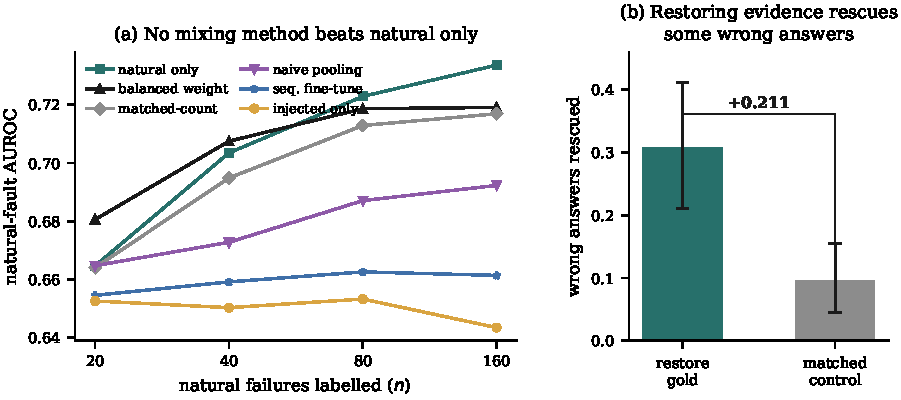
\includegraphics[width=\textwidth]{fig4_budget_causal.pdf}
\caption{(a) Natural-fault AUROC against labelled natural failures, over $40$ query-level
draws. (b) Rescue rates under gold restoration and a length-matched placebo.}
\label{fig:budget}
\end{figure}

A naive comparison would be confounded: thousands of synthetic rows against twenty natural ones
dominate any pooled objective by count alone. We compare six protocols on identical folds ---
synthetic only, natural only, naive pooling, balanced domain weighting, sequential fine-tuning
and matched-count augmentation --- and report paired differences against natural-only.

No protocol significantly outperforms natural-only at any budget. Naive pooling, balanced
weighting and matched-count are statistically indistinguishable from natural-only throughout;
balanced weighting is numerically ahead at $n{=}20$ ($+0.016$ \ci{-0.042}{+0.097}). Only
synthetic-only and sequential fine-tuning become significantly worse, from $n{=}80$
($-0.070$ \ci{-0.105}{-0.010} and $-0.060$ \ci{-0.156}{-0.000}). At $n{=}160$ synthetic-only
trails by $-0.090$ \ci{-0.124}{-0.035}. This does not support the broader claim that twenty
real labels beat thousands of synthetic ones; the gap at $n{=}20$ is not significant. We make
no claim about annotation cost, which we did not measure.

\section{Detection against external detectors}
\label{app:detection}

\begin{table}[h]
\centering\small
\caption{Detection AUROC on the \textsc{decoupled} arm under identical query-disjoint folds.
Best per row in bold; the all-features column indicates the size of the coupling correction.}
\begin{tabular}{@{}llcccccc@{}}
\toprule
Tier & Family & \textsc{decoupled} & \textsc{nli-large} & \textsc{nli} & \textsc{judge} & \textsc{trivial} & \emph{(all feat.)} \\
\midrule
T0 & retrieval  & \best{0.748} & 0.497 & 0.475 & 0.635 & 0.698 & \emph{0.748} \\
T0 & source     & \best{0.667} & 0.522 & 0.564 & 0.538 & 0.514 & \emph{0.675} \\
T0 & tool       & 0.473 & 0.527 & 0.478 & 0.489 & \best{1.000} & \emph{1.000} \\
T0 & grounding  & 0.469 & 0.795 & 0.570 & \best{0.954} & 0.476 & \emph{1.000} \\
T1 & retrieval  & \best{0.864} & 0.489 & 0.501 & 0.652 & 0.699 & \emph{0.864} \\
T1 & source     & \best{0.963} & 0.759 & 0.605 & 0.808 & 0.633 & \emph{0.968} \\
T1 & tool       & 0.495 & \best{0.536} & 0.477 & 0.494 & 0.562 & \emph{0.990} \\
T1 & grounding  & 0.474 & 0.748 & 0.558 & \best{0.772} & 0.516 & \emph{0.608} \\
T2 & retrieval  & \best{0.576} & 0.516 & 0.475 & 0.526 & 0.528 & \emph{0.575} \\
T2 & source     & \best{0.763} & 0.618 & 0.538 & 0.616 & 0.573 & \emph{0.782} \\
T2 & tool       & 0.472 & 0.491 & 0.482 & 0.487 & \best{0.516} & \emph{0.476} \\
T2 & grounding  & 0.483 & \best{0.700} & 0.557 & 0.691 & 0.520 & \emph{0.551} \\
\bottomrule
\end{tabular}
\end{table}

Combining detectors does not help. Under a paired cluster bootstrap on pooled out-of-fold
predictions, $10$ of $36$ union comparisons are significant: eight are regressions, all on
grounding (largest $-0.135$ \ci{-0.156}{-0.113}), and two are small gains. Adding eleven
features blind to grounding dilutes the one or two that are not, so the recommendation is to
route by fault family rather than pool.

\section{The full injector ladder}
\label{app:ladder}

\begin{table}[h]
\centering\small
\caption{All twelve (tier, family) operations. Each injector declares how much of the pipeline
must be re-executed downstream.}
\begin{tabular}{@{}llp{7.6cm}@{}}
\toprule
Family & Tier & Operation \\
\midrule
\texttt{query\_retrieval} & T0 & Reverse the word order of the query. \\
 & T1 & Random dropout of $\approx 50\%$ of query tokens. \\
 & T2 & Delete one high-information content word, chosen by seeded RNG from the three longest. \\
\midrule
\texttt{source\_degradation} & T0 & Prefix the passage with \texttt{"OUTDATED "}. \\
 & T1 & Exchange the selected and rejected passage sets. \\
 & T2 & Keep the top passage; replace the remainder with near-miss distractors. \\
\midrule
\texttt{tool\_invocation} & T0 & Call an unregistered tool name. \\
 & T1 & Emit a malformed expression that really executes and errors. \\
 & T2 & Emit a valid expression with two operands transposed. \\
\midrule
\texttt{grounding} & T0 & Swap in a donor answer from another query. \\
 & T1 & Substitute an entity in the model's own answer. \\
 & T2 & Generator rewrites its answer so one RNG-chosen detail is unsupported. \\
\bottomrule
\end{tabular}
\end{table}

\section{Matched-effect contrasts and tier contrasts}
\label{app:matched}

\begin{table}[h]
\centering\small
\caption{Matched-effect mechanism identification (\textsc{decoupled} arm). Contrasts involving
\texttt{donor} are reported for completeness; \texttt{donor} draws from an unrelated query and
is topically off-subject, so it is not the basis of any claim.}
\begin{tabular}{@{}lccc@{}}
\toprule
\texttt{source\_degradation} & \texttt{rank}--\texttt{lexical} & \texttt{rank}--\texttt{donor} & \texttt{lexical}--\texttt{donor} \\
\midrule
 & $\mathbf{0.633}$ & $0.989$ & $0.984$ \\
\midrule
\texttt{grounding} & \texttt{dict}--\texttt{distractor} & \texttt{dict}--\texttt{donor} & \texttt{distractor}--\texttt{donor} \\
 & $0.507$ & $0.507$ & $0.499$ \\
\bottomrule
\end{tabular}
\end{table}

\begin{table}[h]
\centering\scriptsize
\caption{Declared severity balance for the defensible rank--lexical source contrast. Absolute
standardised mean differences are shown before and after clipped cross-fitted propensity
weighting.}
\label{tab:severity-balance}
\begin{tabular}{@{}lcc@{}}
\toprule
Severity variable & Before & After \\
\midrule
answer similarity & .029 & .002 \\
answer token-length change & .018 & .002 \\
answer character-length change & .011 & .010 \\
changed-token count & .016 & .006 \\
correctness change & .009 & .001 \\
answer token-F1 change & .041 & .004 \\
context token-length change & .320 & .014 \\
question--context overlap & .374 & .002 \\
\bottomrule
\end{tabular}
\end{table}

Severity-only AUROC is $.628$ \ci{.604}{.653}. After reweighting, the decoupled mechanism
probe is $.607$ \ci{.576}{.639}; weights range from $.603$ to $1.966$. The signal attenuates
but remains beyond $D=.05$, while maximum imbalance falls from $.374$ to $.014$.

\begin{table}[h]
\centering\small
\caption{Within-family pairwise \emph{tier} discrimination (\textsc{decoupled}). These do not
hold the semantic effect fixed and are superseded above where a matched construction exists.}
\begin{tabular}{@{}lccc@{}}
\toprule
Family & T0--T1 & T0--T2 & T1--T2 \\
\midrule
\texttt{source\_degradation} & $0.957$ & $0.768$ & $0.949$ \\
\texttt{query\_retrieval}    & $0.813$ & $0.717$ & $0.801$ \\
\texttt{tool\_invocation}    & $0.586$ & $0.542$ & $0.541$ \\
\texttt{grounding}           & $0.499$ & $0.512$ & $0.500$ \\
\bottomrule
\end{tabular}
\end{table}

\section{Probe-family sensitivity}
\label{app:probes}

Discrimination scale $D$ under four model families on identical query-disjoint folds, untuned.
No non-linear family exceeds the linear probe by more than $+0.038$, so the negative results in
Sections~\ref{sec:artifact} and~\ref{sec:ecological} are not artifacts of linearity.

\begin{center}
\small
\begin{tabular}{@{}lcccc@{}}
\toprule
Condition & linear & RBF-SVM & GBM & MLP \\
\midrule
T0 retrieval & $0.454$ & $0.241$ & $0.373$ & $0.324$ \\
T0 source    & $0.301$ & $0.295$ & $0.206$ & $0.286$ \\
T1 retrieval & $0.655$ & $0.567$ & $0.607$ & $0.528$ \\
T1 source    & $0.708$ & $0.554$ & $0.536$ & $0.626$ \\
T2 retrieval & $0.224$ & $0.142$ & $0.005$ & $0.128$ \\
T2 source    & $0.145$ & $0.112$ & $0.182$ & $0.159$ \\
\bottomrule
\end{tabular}
\end{center}

\section{Equivalence margin sensitivity}
\label{app:delta}

Query-matched C2ST under the external representation. Only at $\delta = 0.20$ do most
conditions pass, so the conclusion in Section~\ref{sec:ecological} is not an artifact of a
strict margin: it holds across every margin we consider defensible.

\begin{center}
\small
\begin{tabular}{@{}lcccc@{}}
\toprule
Condition & $\delta{=}0.05$ & $\delta{=}0.10$ & $\delta{=}0.15$ & $\delta{=}0.20$ \\
\midrule
T0 retrieval & fail & fail & fail & pass \\
T1 retrieval & fail & fail & fail & pass \\
T2 retrieval & fail & fail & fail & pass \\
T0 source    & fail & fail & fail & pass \\
T1 source    & fail & fail & fail & fail \\
T2 source    & fail & fail & fail & fail \\
\bottomrule
\end{tabular}
\end{center}

\clearpage
\section{Scale and reproducibility}
\label{app:scale}

The primary HotpotQA/GSM8K campaign contains $24{,}000$ traces: E1 ($200$ clean), E3
($5{,}000$; $200$ queries, three seeds, probe training) and E4 ($18{,}800$; $800$ disjoint
queries, five seeds, test), generated in $15.2$ A6000 GPU-hours. Additional versioned artifacts
contain $7{,}000$ 2Wiki traces, $1{,}400$ at HotpotQA $k{=}3$, $2{,}352$ matched-effect traces
and $600$ released AEGIS rows. The 2Wiki manifest records exactly $7{,}000/7{,}000$ expected
traces; its 200 pilot IDs are disjoint from the 1,000 confirmatory IDs.

Every run has a YAML config, seed and saved query IDs; folds and resampling use query/task
groups. Traces are content-addressed, result JSONs are versioned rather than overwritten, and
raw out-of-fold predictions plus reproducible bootstrap/permutation seeds are retained. The
AEGIS repository commit is pinned above. A machine-readable experiment registry and a separate
claim freeze record the statistic, threshold and confirmatory/diagnostic/post-hoc status. An
invalid source-matching rerun that inherited stale clean metrics is retained under an explicit
\texttt{invalid\_} filename and excluded from every figure and claim. Figures are regenerated
from result JSONs; a verification script checks every number added in this revision against
those files. The released suite currently collects $37$ test cases across seven test modules,
including $23$ parametrized negative-control cases.

\begin{center}
\captionof{table}{Artifact registry for the analyses added or materially changed in this
revision. ``Primary'' means the contrast and interpretation were frozen before the
confirmatory run; the AEGIS mechanism contrast is retained as a diagnostic without a V2
verdict.}
\label{tab:artifact-registry}
\scriptsize
\begin{tabular}{@{}p{2.3cm}p{2.0cm}p{1.1cm}p{2.0cm}p{4.25cm}@{}}
\toprule
Analysis & Rows / groups & Unit & Status & Primary result artifact \\
\midrule
Hotpot/GSM8K validity campaign & $24{,}000$ / $800$ test queries & query & rebuilt confirmatory &
\path{E4_validity_audit_v2.json} \\
Effect-matched V2 & $2{,}352$ / $200$ queries & query & primary + declared robustness &
\path{matched_effect_source_v3.json}; \path{matched_effect_grounding.json} \\
Hotpot query-matched V3 & $71$ natural groups; five synthetic seeds & query & corrected primary &
\path{c2st_matched_v2.json} \\
Hotpot V4 uncertainty & seven candidates, T0--T2 & query & primary bootstrap &
\path{decision_validity_v3.json} \\
2Wiki V3/V4 replication & $7{,}000$ / $1{,}000$ confirmatory queries & query & preregistered replication &
\path{2wiki_c2st_matched_v3.json}; \path{2wiki_decision_validity_v3.json} \\
Causal restoration & $90$ Hotpot; $187$ 2Wiki interventions & query & preregistered intervention &
\path{counterfactual_v2.json}; \path{2wiki_counterfactual_v3.json} \\
External AEGIS audit & $600$ / task-disjoint folds & task & primary V1; diagnostic V2 &
\path{external_aegis_audit_v3.json} \\
Hotpot $k{=}3$ & $1{,}400$ traces & query & operating-point replication &
\path{k3_decision_validity_v2.json} \\
\bottomrule
\end{tabular}
\end{center}

\paragraph{Reproduction order.}
The intended sequence is (1) validate trace manifests and query-ID disjointness, (2) rebuild
features from immutable traces, fitting imputation and scaling only within each training fold,
(3) emit raw out-of-fold predictions before any bootstrap or permutation summary, (4)
regenerate tables and figures from the versioned JSONs, and (5) run
\path{scripts/verify_revision_numbers.py} before compiling the manuscript. Expensive trace
generation is therefore separable from the deterministic analysis/verification pass. The
submission bundles copy the same four vector figures and strengthened appendix; venue-specific
sources change framing and page budget, not numerical evidence.

\paragraph{Automated failure guards.}
The test suite checks that all four families produce distinct tiers and vary with seed, that
the hardened tool fault leaves no tool-health flag, source degradation does not pin QCM to a
sentinel, no evaluator arm contains labels, missing values remain missing until fold-fitted
imputation, duplicate metrics are rejected, seed replicas collapse under deduplication, and
family labels cannot encode tiers. Additional tests require content-addressed artifacts,
real grounding donors, held-out sample sizes for headline results, a declared label-free
severity vector whose weighting reduces imbalance, clean-metric invalidation after an
intervention, explicit AEGIS-field exclusions, stable task grouping, shared queries for V4,
and winner/regret recomputation inside every bootstrap resample. These guards encode the two
self-audit failures as regressions that future changes must not reintroduce.


\end{document}
